In this section we informally introduce \lang{} and the concepts needed to combine LIO and FLAM. Section~\ref{sec:calculus} will then formalize the intuitions presented in this section.

Given a named principal $n \in \Nameset$ we call $n$ a \emph{node} when referring to the machine executing code on $n$'s behalf. We assume each named principal has a corresponding machine executing code on its behalf.

The node $n$ starts off with a current label $\conf{\bot} \wedge \integ{n}$\footnote{We follow the convention of \cite{Arden:2015:FA:2859845.2859998} and omit projections of the $\bot$ principals} and a clearance label $\conf{n} \wedge \integ{\bot}$. Figure~\ref{fig:node-info-flow} illustrates a system running \lang{} with two nodes $n$ and $m$. Node $n$ starts off with a current label $\integ{n}$ and clearance $\conf{n}$, and similarly for $m$. As evaluation proceeds the current label of node $n$ and $m$ will move to the right, but the current label will never enter the white region.

\begin{figure}
    \centering
    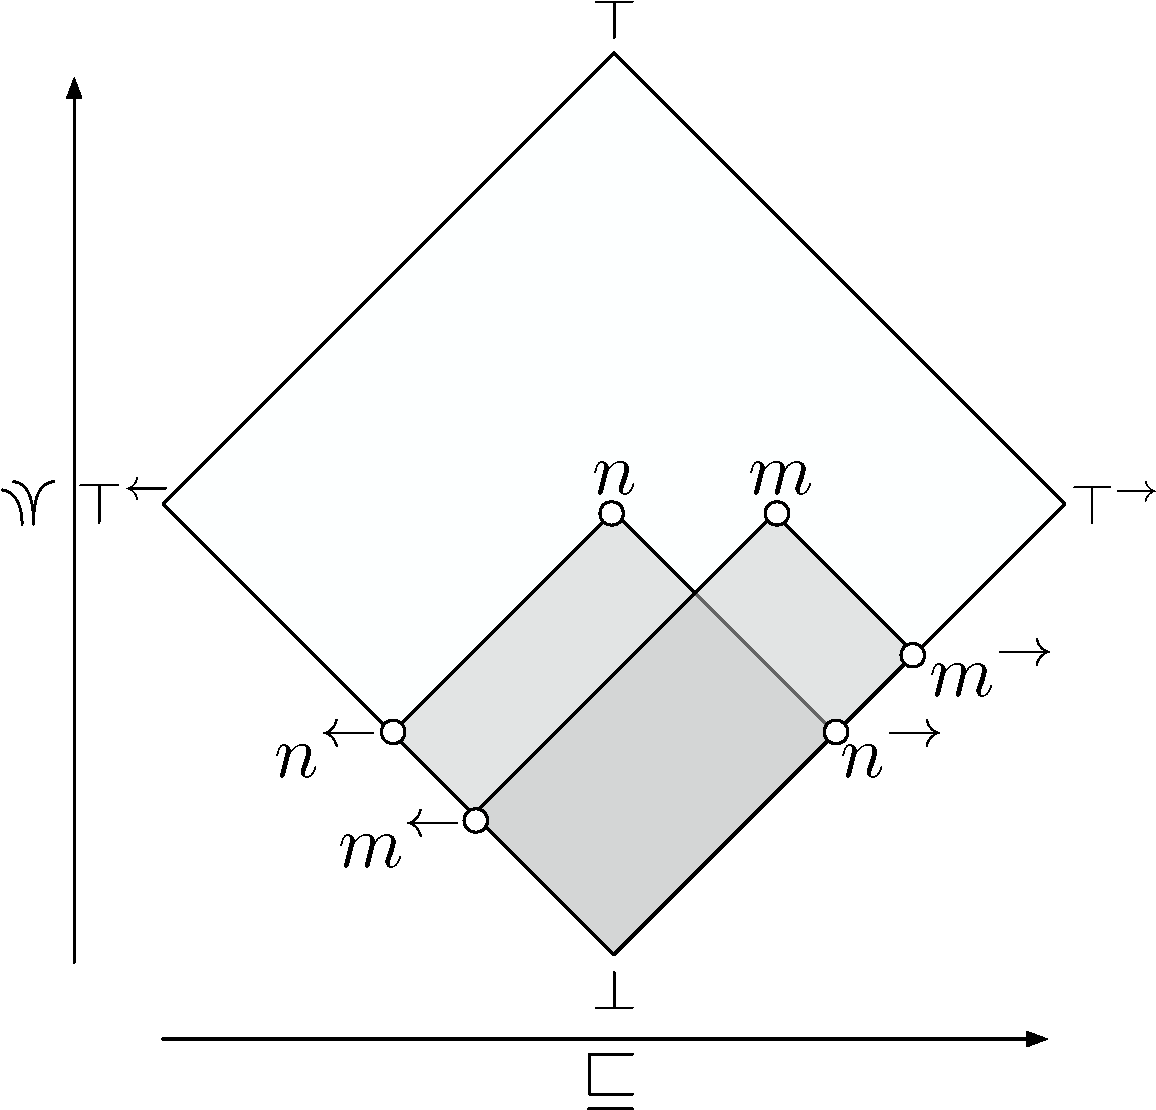
\includegraphics[scale=0.25]{Illustrations/multi-node.pdf}
    \caption{As nodes $n$ and $m$ performs computations their current labels will float from the left-most point to the right-most point in the lattice.}
    \label{fig:node-info-flow}
\end{figure}

We now explore concepts in \lang{} using the named principals $n$ and $m$.

\paragraph{Remote Procedure Calls}
Nodes in \lang{} communicate by remote invocation of functions on different machines. We annotate functions with the node on which the function should be evaluated. That is, the application $\app{(\abs{n}{p}{x}{\expr})}{\expr'}$ denotes a function $\abs{n}{p}{x}{\expr}$ located on machine $n$ should be evaluated with argument $\expr'$ and the returned expression will be given label $p$. For instance, the expression
\begin{lstlisting}
((*@$\lambda^{n}_{p}$@*) x . not x) b >>= (*@$\lambda^{m}_{m}$@*) y . unlabel y
\end{lstlisting}
computes the negation of the boolean $b$ on node $n$ and returns the result as a labeled value with label $p$, which is then unlabeled on node $m$. After receiving the labeled value computed by node $n$, node $m$ needs to unlabel the value to use it. To do this \TODO{node m uses the unlabel operation, which checks that m has sufficient authority to do this.}

\BRAINDUMP{
Talk about:
\begin{itemize}
    \item RPC
    \item Nodes
    \item Proof search
    \item Delegations
    \item Strategies
\end{itemize}}